\documentclass[conference]{IEEEtran}
\IEEEoverridecommandlockouts
% The preceding line is only needed to identify funding in the first footnote. If that is unneeded, please comment it out.
\usepackage{cite}
\usepackage{algorithm}
\usepackage{amsmath,amssymb,amsfonts}
\usepackage{algorithmic}
\usepackage{graphicx}
\usepackage{textcomp}
\usepackage{amssymb}
\usepackage{physics}
\usepackage{amsmath}% http://ctan.org/pkg/amsmath
\newcommand\sufr[3][0pt]{$\rule{0pt}{\dimexpr#1+1.4ex\relax}^\frac{#2}{#3}$}
\usepackage{xcolor}
\def\BibTeX{{\rm B\kern-.05em{\sc i\kern-.025em b}\kern-.08em
    T\kern-.1667em\lower.7ex\hbox{E}\kern-.125emX}}
\begin{document}

\title{Evolutionary Quantum Transition (EQUATe): A Novel Solution to Optimization Problems \\
% {\footnotesize \textsuperscript{*}Note: Sub-titles are not captured in Xplore and
% should not be used}
% \thanks{Identify applicable funding agency here. If none, delete this.}
}

% \author{\IEEEauthorblockN{1\textsuperscript{st} Given Name Surname}
% \IEEEauthorblockA{\textit{dept. name of organization (of Aff.)} \\
% \textit{name of organization (of Aff.)}\\
% City, Country \\
% email address}
% \and
% \IEEEauthorblockN{2\textsuperscript{nd} Given Name Surname}
% \IEEEauthorblockA{\textit{dept. name of organization (of Aff.)} \\
% \textit{name of organization (of Aff.)}\\
% City, Country \\
% email address}
% \and
% \IEEEauthorblockN{3\textsuperscript{rd} Given Name Surname}
% \IEEEauthorblockA{\textit{dept. name of organization (of Aff.)} \\
% \textit{name of organization (of Aff.)}\\
% City, Country \\
% email address}
% \and
% \IEEEauthorblockN{4\textsuperscript{th} Given Name Surname}
% \IEEEauthorblockA{\textit{dept. name of organization (of Aff.)} \\
% \textit{name of organization (of Aff.)}\\
% City, Country \\
% email address}
% \and
% \IEEEauthorblockN{5\textsuperscript{th} Given Name Surname}
% \IEEEauthorblockA{\textit{dept. name of organization (of Aff.)} \\
% \textit{name of organization (of Aff.)}\\
% City, Country \\
% email address}
% \and
% \IEEEauthorblockN{6\textsuperscript{th} Given Name Surname}
% \IEEEauthorblockA{\textit{dept. name of organization (of Aff.)} \\
% \textit{name of organization (of Aff.)}\\
% City, Country \\
% email address}
% }

\maketitle

\begin{abstract}
Quantum Computing (QC) has often been touted as an esoteric and terrifying field of computing research. However, the possible advantages offered by the inherent quantum fundamentals beseeches extensive additional ventures into this field. Likewise, Evolutionary Computing (EC) offers a multi-pronged approach by deploying several candidates into the search space with constraints guiding the search process. In this paper, we present Evolutionary Quantum Transition (EQUATe) to provide a unique solution to solving Multi-Optimization Objective Problems (MOOPs) using concepts borrowed from QC and EC. The combination leverages compute power to explore the space of candidate solutions by introducing smarter techniques. The solution so obtained provides the optimal transition solution with an automated circuit selection process which can be attributed to the amazing capabilities of QC and EC. 
\end{abstract}

\begin{IEEEkeywords}
Quantum Computing, Evolutionary Computing, MOOPs, EQUATe, State Transition
\end{IEEEkeywords}

\section{Introduction}

Majority of the problems faced in any aspect of computer science, in one way or another, involves a catch-22 of functional optimization. Entire fields have been dedicated to solving a generic version of this issue. The most common method of dealing with optimization problems is to be in collaboration with another interdisciplinary frontier acting in the capacity of a helper function. 

\subsection{Modeling an Optimization Problem}
Before any optimization can be performed, a mathematical or computational model for the problem must be prepared \cite{hara}. The quality of the model is just as crucial to the optimization task as the techniques employed. Drafting the model requires explicitly stating the variables, constraints, and objective functions involved followed by the selection of an appropriate algorithm for the search process. 

\subsection{Problem Formalization}
The optimization problems considered in this paper belong to the family of Multi-Objective Optimization Problems (MOOPs)\cite{mul}. Any other problem format can be derived from this main branch. A general MOOP is defined in Equation :


\begin{equation}
Optimize \{f\textsubscript{1}(x), f\textsubscript{2}(x), \dots, f\textsubscript{k}(x)\}
\end{equation}

where $f\textsubscript{i}(x)$ is the $i\textsuperscript{th}$ sub-problem subject to certain constraints. The decision vector $X$ = ($x\textsubscript{1}, x\textsubscript{2}, \dots, x\textsubscript{n}$) belong to a nonempty feasible region $S$. The objective solution vector $Z$ =  $(f\textsubscript{1}(x), f\textsubscript{2}(x), \dots, f\textsubscript{k}(x))$ represents the required mapping in the feasible objective region $Z$. 

Such a mapping is considered to be optimal if none of the individual components can be improved without degradation of at least one other component and such a solution vector is called a Pareto optimal solution \cite{pare}. An ideal objective vector $z\textsuperscript{*}$ can be obtained by minimizing every objective function individually subject to $S$. A vector strictly better than $z\textsuperscript{*}$ is called a utopian objective vector $z\textsuperscript{**}$. Similarly, the upper bounds of the Pareto Optimal set to constitute a nadir objective vector $z\textsuperscript{nad}$. Once the variables are decided, we can embark upon finding a solution to the optimization problem. Various techniques can be chosen to solve the problem. The most popular ones are described in the next section. 

\section{Computing Methology}

Once the problem statement is defined and the model is formulated, a computing technique must be selected for solving the MOOP. Historically, three main verticals have stood out as prime candidates for solving MOOPs. They been described in Table $\ref{tab:1}$. 

\begin{table*}[!t]
\caption{\textsc{Computing Methodologies}}
\label{tab:1}
\centering
{
\begin{tabular}{| c | c | c | c |}
\hline
\textbf{Method} & \textbf{Key Points} & \textbf{Advantages} & \textbf{Disadvantages} \\
\hline
& Use of bits for information & Intuative, Can be modelled at & High space complexity, susceptible\\
Classical Computing (CC)&transmission, Deterministic Modeling, &present, Easier state transition,& to noise, Limited parallelism,\\
&Used to day-to-day tasks& Resources are available on-the-go & Slow convergence rate\\
\hline
& Multiple search candidates, & Faster convergence to solution, & Computationally Intensive \\
Evolutionary Computing (EC)& Concepts borrowed from nature,& Independent of complexity of problem,& Sensitive to parameter tuning,\\
&Easily understandable&Mathematical representation optional& Optimal solution not guarenteed\\
\hline
& Use of Quantum mechanics, & Rapid solution search, & Quantum Mechincial knowledge as \\
Quantum Computing (QC)& Bra-ket representation instead of bits, & Space conservation, & a prerequisite, Not Intuative, \\
&Stochastic Modeling&Unprecedented Computational abilities&Lack of Quantum resources\\
\hline
\end{tabular}
}
\end{table*}

\subsection{Why go Quantum?}

% The field of applied quantum mechanics is still unexplored for the best part. However, there are certain applications in which QC outperforms CC. Consider Shor's algorithm \cite{shor} and RSA \cite{rsa}, both of which are used for encryption. Basically, the encryption of any form of data transmitted over the Internet relies immensley on factorization of a huge number. This process is extremley ardous for a non-quantum computer, with the best known factoring technique requiring an amount of time proportional to 2$\textsuperscript{n\textsuperscript{\sufr{1}{3}}log(n)\textsuperscript{\sufr{2}{3}}}$ 
% , where $\textit{n}$ is the number of digits in the number to be factored \cite{guo}. Meanwhile Shor's Quantum algorithm requires time proportional to only $n\textsuperscript{2}log(n)log(log(n))$ \cite{ham}. 

QC utilizes major quantum phenomena such as superposition, quantum entanglement, the principle of uncertainty among others \cite{az}, for improving existing search and optimization techniques. The time required for processing a search request decreases exponentially in a QC environment as multiple states are entangled.  
% according to Moore's Law the size of computational units shrinks at an exponential rate as the number of transistors on a chipset increases every year. Even after accounting for physical constraints, a time will come when operations will be conducted on an atomic scale which quantum physics dominates classical physics. As a result, understanding QC and applying them in a virtual landscape to get a sense of their possibilities is a must. 

\subsection{Using Evolutionary Algorithms}

Evolutionary Algorithms (EA) \cite{vik} encompass a wide array of research ideas stemming from general principles of genetics and the theory of evolution. Models are developed to illustrate the behavior of naturally occurring phenomena, develop these algorithms, and test out the application of the corresponding theory. The general process of any EA is depicted in figure \ref{p1}. 

\begin{figure}[!t]
\centering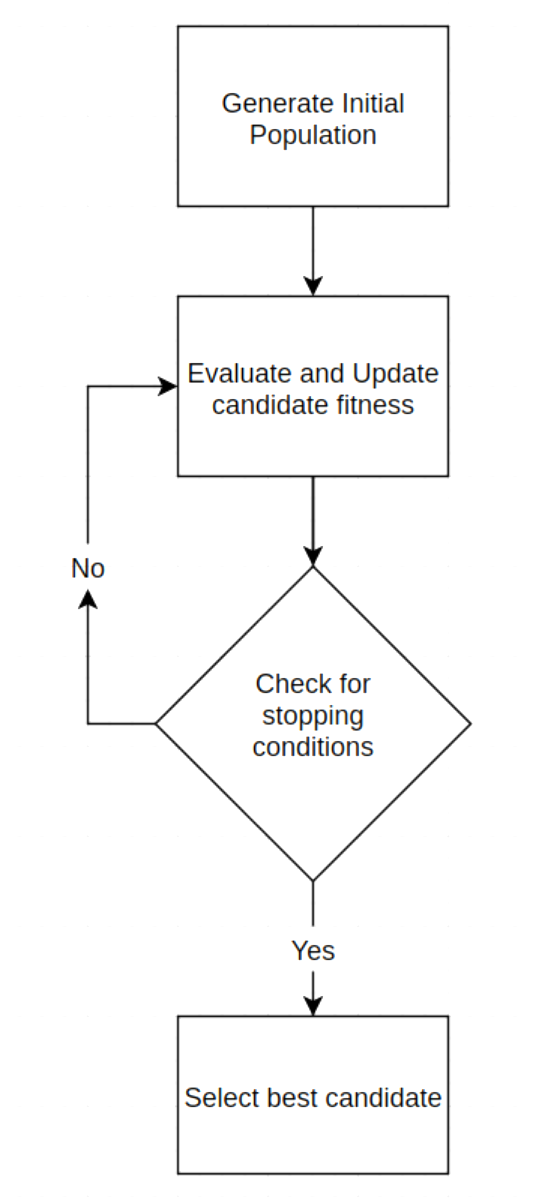
\includegraphics[height=6.75cm]{p1.png}
\caption{General Flow of Evolutionary Algorithms}
\label{p1}
\end{figure}

\subsection{EQUATe: A Novel Ensemble}
As we have seen, each vertical offers it's own advantages and disadvantages when it comes to solving an optimization problem. A trade-off exists between CC and QC when it comes to delivering quality results in a reduced time frame and availability of resources to implement the search process. Meanwhile, EC offers a multi-pronged approach to the search process by applying certain constraints and operators which results in the emergence of the best results with a decreased time complexity. EQUATe borrows the most promising concepts from QC and EC to provide a new front to solving optimization problems. The space-saving capabilities offered by QC are excellent additions to EQUATe. Likewise, the evolutionary model offered by EC boosts the search process. The general MOOP is a relatively broad set of problems, with each problem requiring certain tweaks to the solution search process. In this paper, we narrow down the MOOPs to a specific case i.e, Design a circuit to achieve state $j$ from $i$ with multiple cost considerations. 
% \subsection{Computing Methodologies}
% 
% Most form of computational algorithms in the present day, are executed on a conventional computer. The fundamental notation used for differentiating Classical Computing (CC) and QC \cite{nara} is the basic unit of information. While classical computers use bits 0 and 1, quantum computers use "one of" two computational basis states. The label awarded to these states is "bra-ket" notation i.e, state $\ket{0}$ or $\ket{1}$. Bits are assigned states 0 or 1 deterministically and independently. However, qbuits can exist in a superposition state of $\alpha\textsubscript{0}$$\ket{0}$ + $\alpha\textsubscript{1}$$\ket{1}$, where $\alpha{0}$ and $\alpha{1}$ are complex numbers, such that $|\alpha\textsubscript{0}|\textsuperscript{2}$ + $|\alpha\textsubscript{1}|\textsuperscript{2}$ = 1.
% 


% \section{Methodology}
% 
% Our paper provides an insight into the ensemble of both the previously mentioned techniques and preparing algorithms for a future where quantum computers replace traditional computers as commonplace machines. 
% \subsection{Existing Convention}
% 
% Consider the previously stated problem; Assume the position of a process $\textit{P}$ in a finite state system of $\textit{n}$ states at time $\textit{t}$ to be $\textit{x\textsubscript{i}}$. Create a general procedure to reach position $\textit{x\textsubscript{j}}$ at time $\textit{t+1}$.
% 
% The conventional process would involve declaration of a register of size $\textit{n}$ and listing out all possible combinations for reaching state $\textit{x\textsubscript{j}}$ along with the costs. This would be followed by creation of a logical circutry of gates mapping the input state to the output state using boolean primitives. The entire process could still be automated using certain advanced algorithms. However, the memory utilization will not be optimal as all possible state transitions must be considered before building the circuit. Figure $\ref{p2}$ displays the state table, state diagram and accompanying circuit diagram for a D flip flop. Notice that all possible states for the input have been mentioned in the state table. This constitues a huge waste of memory as majority of the inputs are never encountered and some states could be invalid. QC aims to reduce this inefficiency between making all the states dependent on each other. 
% 
\begin{figure}[!b]
\centering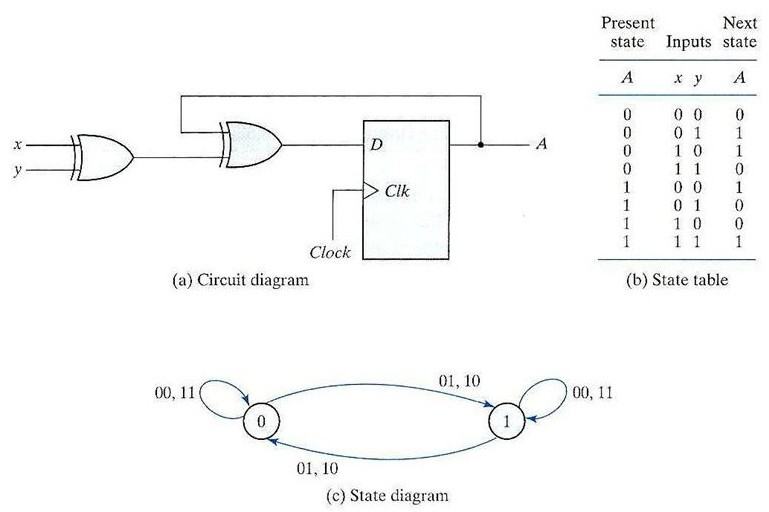
\includegraphics[width=8cm]{ss.jpg}
\caption{States for D flip flop}
\label{p2}
\end{figure}
% 
% \subsection{Applied Quantum Mechanics}
% Classicial state transitions cannot fathom superposition and hence will always be fixated on one fixed state. For the D flip flop example, the number of inputs are two and hence the number of output states is $2\textsuperscript{2}$ for each starting state. The 4 possible states can be represented as an one-hot encoded vector with each bit representing the state of the output. For example, the vector shown below represents state 00 for an input state of 0.
% $$
% \begin{bmatrix} 
% 1&0&0&0\\
% \end{bmatrix}
% \quad
% $$
% 
% Quantum Mechanics is a generalized extension of classical method. The first generalization comes in the form of the temporal values of the elements of the matrix. In QC qubits are utilized instead of bits and as a result the state vectors are variables. Instead of 0 and 1, state vector can be constituted of complex numbers which meet the condition of unitarity. For any matrix $\textit{M}$ to be an unitarity matrix, the only necessary condition is shown in Equation $\ref{eq:1}$ where $M\textsuperscript{$\dagger$}$ is the Hermitean adjoint of $\textit{M}$ and $\textit{I}$ is the identity matrix. 
% {\scriptsize
% \begin{equation}
% \label{eq:1}
% M\textsuperscript{$\dagger$}M = MM\textsuperscript{$\dagger$} = I
% \end{equation}
% }
% 
% To facilitate the design of circuitry of state diagrams, QC introduces a set of gates to utilize the power of quantum mechanics \cite{qg}. The noteworthy ones are mentioned below:
% 
% \begin{itemize}
% \item QNOT: This gate is the quantum extension of the controlled NOT gate in CC. A controlled NOT gate performs the inversion operation on the right-most bit of a vector iff the left-most bit is 1. A 1-bit QNOT gate is depicted as follows:
% $$
% \begin{bmatrix} 
% 0&1\\
% 1&0\\
% \end{bmatrix}
% \quad
% $$
% \item SRN: The application of Square Root of NOT puts a qubit into a state of equal superposition through controlled randomization based on the qubit's past state. A 1-bit SRN is shown below:
% $$
% \begin{bmatrix} 
% \frac{1}{\sqrt{2}}&\frac{-1}{\sqrt{2}}\\
% \frac{1}{\sqrt{2}}&\frac{1}{\sqrt{2}}\\
% \end{bmatrix}
% \quad
% $$
% \item Swap: As the name suggests, this gate is used to swap the states of two qubits and is represented as:
% $$
% \begin{bmatrix} 
% {1}&{0}&{0}&{0}\\
% {0}&{0}&{1}&{0}\\
% {0}&{1}&{0}&{0}\\
% {0}&{0}&{0}&{1}\\
% \end{bmatrix}
% \quad
% $$
% \item Parameterized Rotation: This is a family of 1-qubit rotations parameterized by angle $\theta$ and is given by:
% $$
% \begin{bmatrix} 
% cos(\theta)&sin(\theta)\\
% -sin(\theta)&cos(\theta)\\
% \end{bmatrix}
% \quad
% $$
% \end{itemize}
% 
% \subsection{Applied Evolutionary Operators}
% 
% EA have been used extensively for complex optimization problems due to quality results even with a lack of mathematical representation, convexity and continuity. They apply a stochastic method and hence expedite the search process. However, EA are not without their flaws which include a probabilistic convergence to the global optima. 
% 
% In this paper, we follow a genetic modified Grey Wolf Optimization (GWO) algorithm \cite{gwo} to obtain and update candidate solutions. GWO follows a hierarchical structure of candidate solution which imitates the behaviour of Grey Wolves as observed in nature. The structure of $\alpha$, $\beta$, $\delta$ and $\omega$ labelled wolves. The $\alpha$ wolves are responsible for finding the global optimum whilst being guided by the $\beta$ wolves. The $\delta$ and $\omega$ provide secondary assistance to the leaders and hence maitain the dominant structure. After each search iteration, genetic operators like selection, crossover and mutation are applied to every candidate in the structure. The entire process is discribed in Algorithm $\ref{alg:gwo}$
% 
% \begin{algorithm}[t]
% \footnotesize
% \caption{GWO pseudocode}
% \label{alg:gwo}
% \begin{algorithmic}[1]
% \STATE \textbf{Input:} Population size $\textit{n}$, random vectors $\vec{r\textsubscript{1}}$, $\vec{r\textsubscript{2}} \in$ [0,1], initial prey location $\vec{D}$, number of iterations \textit{I}, fitness function $\textit{f}$, coefficient vectors $\vec{A}$, $\vec{C}$ and $\vec{a}$
% \STATE Set $\textit{t}$ = 0
% \FOR{i $\in$ [1,n]}    
% \STATE Generate wolf pack population $\textit{X\textsubscript{i}(t)}$ at instance $\textit{t}$
% \STATE Evaluate each individual against the fitness function
% \ENDFOR
% \STATE Assign $\alpha, \beta, \delta$ titles to the top three solutions
% \STATE Evaluate $\vec{D} = |\vec{C} \cdot \vec{X\textsubscript{p}}(t) - \vec{X}(t)|$
% \FOR{\textit{i} in \textit{I}}
% \FOR{Each individual in $\textit{n}$}  
% \STATE $\vec{X\textsubscript{1}} = \vec{X\textsubscript{$\alpha$}} - \vec{A\textsubscript{1}} \cdot  \vec{D\textsubscript{$\alpha$}}$
% \STATE $\vec{X\textsubscript{2}} = \vec{X\textsubscript{$\beta$}} - \vec{A\textsubscript{2}} \cdot  \vec{D\textsubscript{$\beta$}}$
% \STATE $\vec{X\textsubscript{3}} = \vec{X\textsubscript{$\delta$}} - \vec{A\textsubscript{3}} \cdot  \vec{D\textsubscript{$\delta$}}$
% \STATE Evaluate $\vec{X}(t+1) = \frac{\vec{X\textsubscript{1}} + \vec{X\textsubscript{2}} + \vec{X\textsubscript{3}}}{3}$
% \ENDFOR
% \STATE Update the coefficient vectors $\vec{A}$ and $\vec{C}$
% \STATE $\vec{A} = 2\vec{a} \cdot \vec{r\textsubscript{1}} - \vec{a}$
% \STATE $\vec{C} = 2\vec{r\textsubscript{2}}$
% \STATE Linearly decrease $\vec{a}$ from 2 to 0
% % \STATE Update $\vec{X\textsubscript{$\alpha$}}, \vec{X\textsubscript{$\beta$}}, \vec{X\textsubscript{$\delta$}}$
% \STATE Perform Crossover, Selection and Mutation
% \STATE Increment $\textit{t}$
% \ENDFOR
% \STATE $\vec{X\textsubscript{$\alpha$}}$ corresponds to the global optimum. 
% \end{algorithmic}
% \end{algorithm}
% 
% The genetic operators for a sample candidate in the form of a genomic are explained here following which the process is depicted in Figure :
% \begin{itemize}
% \item Selection: Given a population of potential solutions, selection involves grading these solutions against a fitness function. The selected solutions are cast into the crossover stage.
% \item Crossover: From the selected set of solutions, randomly two solutions are selected and the next generation chromosome is created which shares the best attributes of it's parents.
% \item Mutation: The selected solutions undergo random changes in their composition to promote diversity and increase their changes of converging to the global optimum.
% \end{itemize}
% 
% \begin{figure}[!t]
% \centering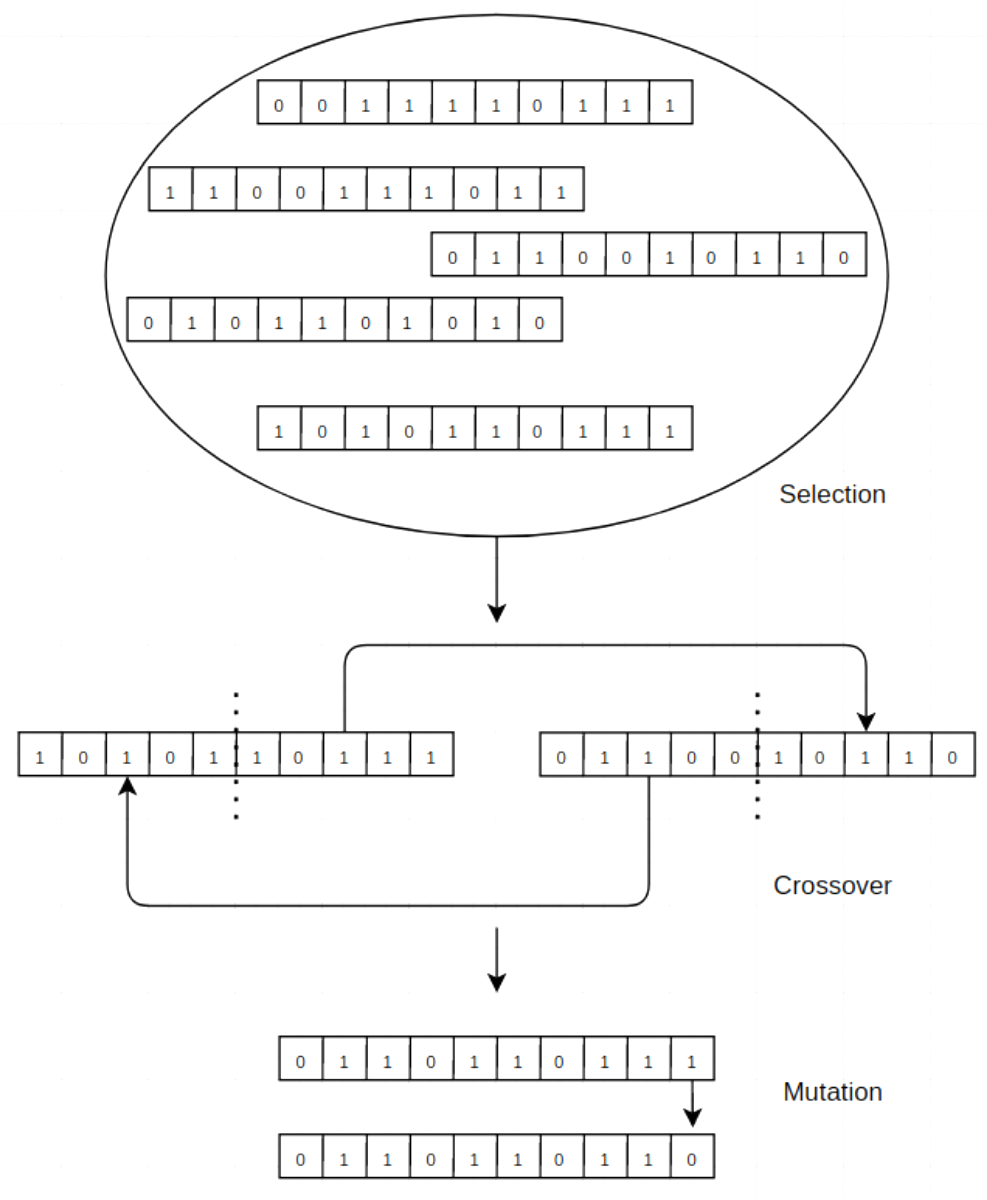
\includegraphics[width=7cm]{p2.png}
% \caption{Genetic Operators}
% \label{p3}
% \end{figure}

\section{Evolutionary Quantum Transition (EQUATe)}

Evolved self-organizing computer programs \cite{self} utilize the techniques described in the previous section to solve problems. In this paper the following general problem structure is considered for demonstrating the capabilities of EQUATe; How to design a circuit to travel from state $\textit{A}$ to state $\textit{B}$? These problem types are called "Oracle Analysis" \cite{oracle} as they require we to determine some property of a valid quantum gate with no prior information on the intermediate states and what combination of gates results in what output. Some of the key terminologies used in the following texts are explained in Table $\ref{tab:2}$



\begin{table}[!t]
\caption{\textsc{Basic Terminology}}
\label{tab:2}
\centering
{
\begin{tabular}{| c | c |}
\hline
Symbol  & Description \\
\hline
$\psi\textsubscript{i}$ & Current State \\ 
$\psi\textsubscript{o}$ & Desired State \\
$\psi\textsubscript{best}$ & Current Best State \\
$\textit{T}$ & Circuit operator\\
$\textit{F}$ & Fitness function\\
$\textit{M}$ & Number of chromosomes\\
$\textit{G}$ & Number of generations\\
$\textit{sel\_tech}$ & Selection Techniques\\
$\textit{cross\_tech}$ & Crossover Techniques\\
$\textit{mut\_tech}$ & Mutation Techniques\\
$\textit{n}$ & Dimensionality of chromosome\\
$\textit{U(n)}$ & Space of all $\textit{n}$ dimensional matrices\\
$\textit{H\textsubscript{cur}}$ & Current Gate Matrix\\
$\textit{H\textsubscript{cur}\textsuperscript{$\dagger$}}$ & Hermitean Adjoint of $\textit{H\textsubscript{cur}}$\\
$\ket{A\textsubscript{k}}(\psi)$ & Orthonormal basis of the environment Hilbert space\\
$p\textsubscript{k}$ & Input mapped to Hilbert space\\
$q\textsubscript{k}$ & Output mapped to Hilbert space\\
\hline
\end{tabular}
}
\end{table}

\subsection{Conventional Approach}
The conventional process would involve a declaration of a register of size $\textit{n}$ and listing out all possible combinations for reaching state $\textit{x\textsubscript{j}}$ along with the costs. This would be followed by the creation of a logical circuitry of gates mapping the input state to the output state using boolean primitives. The entire process could still be automated using certain advanced algorithms. However, the memory utilization will not be optimal as all possible state transitions must be considered before building the circuit. Figure $\ref{p2}$ displays the state table, state diagram, and accompanying circuit diagram for a D flip flop. Notice that all possible states for the input have been mentioned in the state table. This constitutes a huge waste of memory as the majority of the inputs are never encountered and some states could be invalid. QC aims to reduce this inefficiency between making all the states dependent on each other.

\subsection{The EQUATe Approach}

The conventional approach is extremely inefficient and arduous. EQUATe offers an elegant solution by utilizing the best of both worlds. 

\subsubsection{Applied Quantum Mechanics for EQUATe}
Classical state transitions cannot fathom superposition and hence will always be fixated on one fixed state. For the D flip flop example, the number of inputs is two and hence the number of output states is $2\textsuperscript{2}$ for each starting state. The 4 possible states can be represented as a one-hot encoded vector with each bit representing the state of the output. For example, the vector shown below represents state 00 for an input state of 0.
$$
\begin{bmatrix} 
1&0&0&0\\
\end{bmatrix}
\quad
$$

Quantum Mechanics is a generalized extension of the classical method. The first generalization comes in the form of the temporal values of the elements of the matrix. In QC qubits are utilized instead of bits and as a result, the state vectors are variables. Instead of 0 and 1, the state vector can be constituted of complex numbers that meet the condition of unitarity. For any matrix $\textit{M}$ to be an unitarity matrix, the only necessary condition is shown in Equation $\ref{eq:1}$ where $M\textsuperscript{$\dagger$}$ is the Hermitian adjoint of $\textit{M}$ and $\textit{I}$ is the identity matrix. 

\begin{equation}
\label{eq:1}
M\textsuperscript{$\dagger$}M = MM\textsuperscript{$\dagger$} = I
\end{equation}


To facilitate the design of circuitry of state diagrams, QC introduces a set of gates to utilize the power of quantum mechanics \cite{qg}. The noteworthy ones are mentioned below:

\begin{itemize}
\item QNOT: This gate is the quantum extension of the controlled NOT gate in CC. A controlled NOT gate performs the inversion operation on the right-most bit of a vector iff the left-most bit is 1. A 1-bit QNOT gate is depicted as follows:
$$
\begin{bmatrix} 
0&1\\
1&0\\
\end{bmatrix}
\quad
$$
\item SRN: The application of Square Root of NOT puts a qubit into a state of equal superposition through controlled randomization based on the qubit's past state. A 1-bit SRN is shown below:
$$
\begin{bmatrix} 
\frac{1}{\sqrt{2}}&\frac{-1}{\sqrt{2}}\\
\frac{1}{\sqrt{2}}&\frac{1}{\sqrt{2}}\\
\end{bmatrix}
\quad
$$
\item Swap: As the name suggests, this gate is used to swap the states of two qubits and is represented as:
$$
\begin{bmatrix} 
{1}&{0}&{0}&{0}\\
{0}&{0}&{1}&{0}\\
{0}&{1}&{0}&{0}\\
{0}&{0}&{0}&{1}\\
\end{bmatrix}
\quad
$$
\item Parameterized Rotation: This is a family of 1-qubit rotations parameterized by angle $\theta$ and is given by:
$$
\begin{bmatrix} 
cos(\theta)&sin(\theta)\\
-sin(\theta)&cos(\theta)\\
\end{bmatrix}
\quad
$$
\end{itemize}

The process of achieving the target state is discussed in this section. For any test function provided, a set of $\textit{M}$ chromosomes are initialized, and based on the input, $\textit{U(n)}$ is laid out. Consider applying set of quantum operators $\textit{Q\textsubscript{$\mu$}}$ on the quantum register of chromosomes for $\mu \in [1,o]$. The output state $\mu$ for an input qubit chromosome $\ket{\psi\textsubscript{i}}$ using operator $\textit{Q\textsubscript{$\mu$}}$, can be determined in a probabilistic manner as shown in Equation $\ref{eq:2}$

\begin{equation}
\label{eq:2}
Pr(\mu) = \bra{\psi} Q\textsubscript{$\mu$}\textsuperscript{$\dagger$}Q\textsubscript{$\mu$}\ket{\psi}
\end{equation}

Similarly the probability of a required state $\mu$ is given in Equation $\ref{eq:3}$

\begin{equation}
\label{eq:3}
\ket{\mu} = \frac{Q\textsubscript{$\mu$}\ket{\psi}}{\sqrt{Pr(\mu)}}
\end{equation}

Since the states can be unitary i.e $\textit{H\textsubscript{cur}} \cdot$ $\textit{H\textsubscript{cur}\textsuperscript{$\dagger$}} = I$, elements of $\textit{U(n)}$ will have a definite form. For example, any element of $\textit{U(2)}$, say $\textit{T}$, will have the following format for complex inputs $z\textsubscript{1}$ and $z\textsubscript{2}$ seperated by an angle $\theta$:
$$
\begin{bmatrix} 
{z\textsubscript{1}}&{z\textsubscript{2}}\\
{-e\textsuperscript{i$\theta$}z\textsubscript{1}\textsuperscript{*}}&{-e\textsuperscript{i$\theta$}z\textsubscript{2}\textsuperscript{*}}\\
\end{bmatrix}
\quad
$$

Now the problem boils down to selection of a particular configuration of these gates. EA uses this subspace and evolutionary techniques to get from  $\psi\textsubscript{i}$ to $\psi\textsubscript{o}$ in $\textit{G}$ generations. A grid of $\textit{sel\_tech}$, $\textit{cross\_tech}$ and $\textit{mut\_tech}$ is created and all the matrices are graded according to $\textit{F}$. This step leads into Algorithm $\ref{alg:gwo}$ which provides the optimal circuit configuration to reach $\psi\textsubscript{best}$, that is closest to $\psi\textsubscript{2}$. The entire process is descibed in Algorithm $\ref{alg:eq}$. 

\begin{algorithm}[!b]
\footnotesize
\caption{EQUATe}
\label{alg:eq}
\begin{algorithmic}[1]
\STATE \textbf{Input:} $\psi\textsubscript{i}$, $\psi\textsubscript{o}$, $\textit{F}$, $\textit{M}$, $\textit{G}$, $\textit{sel\_tech}$, $\textit{cross\_tech}$ and $\textit{mut\_tech}$
\STATE Identify $\textit{n}$ as dimension of input
\STATE Create a grid encompassing all combinations of $\textit{sel\_tech}$, $\textit{cross\_tech}$ and $\textit{mut\_tech}$
\FOR{Each generation $\textit{G}$}
\STATE Evaluate the chromosomes against $\textit{F}$
\STATE Call Algorithm $\ref{alg:gwo}$ with the grid, $\psi\textsubscript{i}$ and $\psi\textsubscript{o}$ 
\STATE Obtain returned $\psi\textsubscript{best}$
\ENDFOR
\STATE Select the optimal $\psi\textsubscript{best}$
\end{algorithmic}
\end{algorithm}

\subsection{Applied Evolutionary Operators for EQUATe}

EC has been used extensively for complex optimization problems due to quality results even with a lack of mathematical representation, convexity, and continuity. They apply a stochastic method and hence expedite the search process. However, EA is not without their flaws which include a probabilistic convergence to the global optima. 

In this paper, we follow a genetically modified Grey Wolf Optimization (GWO) algorithm \cite{gwo} to obtain and update candidate solutions. GWO follows a hierarchical structure of the candidate solution which imitates the behavior of Grey Wolves as observed in nature. The structure of $\alpha$, $\beta$, $\delta$ and $\omega$ labelled wolves. The $\alpha$ wolves are responsible for finding the global optimum whilst being guided by the $\beta$ wolves. The $\delta$ and $\omega$ provide secondary assistance to the leaders and hence maintain the dominant structure. After each search iteration, genetic operators like selection, crossover, and mutation are applied to every candidate in the structure. The entire process is described in Algorithm $\ref{alg:gwo}$

\begin{algorithm}[t]
\footnotesize
\caption{GWO pseudocode}
\label{alg:gwo}
\begin{algorithmic}[1]
\STATE \textbf{Input:} Population size $\textit{n}$, random vectors $\vec{r\textsubscript{1}}$, $\vec{r\textsubscript{2}} \in$ [0,1], initial prey location $\vec{D}$, number of iterations \textit{I}, fitness function $\textit{f}$, coefficient vectors $\vec{A}$, $\vec{C}$ and $\vec{a}$
\STATE Set $\textit{t}$ = 0
\FOR{i $\in$ [1,n]}    
\STATE Generate wolf pack population $\textit{X\textsubscript{i}(t)}$ at instance $\textit{t}$
\STATE Evaluate each individual against the fitness function
\ENDFOR
\STATE Assign $\alpha, \beta, \delta$ titles to the top three solutions
\STATE Evaluate $\vec{D} = |\vec{C} \cdot \vec{X\textsubscript{p}}(t) - \vec{X}(t)|$
\FOR{\textit{i} in \textit{I}}
\FOR{Each individual in $\textit{n}$}  
\STATE $\vec{X\textsubscript{1}} = \vec{X\textsubscript{$\alpha$}} - \vec{A\textsubscript{1}} \cdot  \vec{D\textsubscript{$\alpha$}}$
\STATE $\vec{X\textsubscript{2}} = \vec{X\textsubscript{$\beta$}} - \vec{A\textsubscript{2}} \cdot  \vec{D\textsubscript{$\beta$}}$
\STATE $\vec{X\textsubscript{3}} = \vec{X\textsubscript{$\delta$}} - \vec{A\textsubscript{3}} \cdot  \vec{D\textsubscript{$\delta$}}$
\STATE Evaluate $\vec{X}(t+1) = \frac{\vec{X\textsubscript{1}} + \vec{X\textsubscript{2}} + \vec{X\textsubscript{3}}}{3}$
\ENDFOR
\STATE Update the coefficient vectors $\vec{A}$ and $\vec{C}$
\STATE $\vec{A} = 2\vec{a} \cdot \vec{r\textsubscript{1}} - \vec{a}$
\STATE $\vec{C} = 2\vec{r\textsubscript{2}}$
\STATE Linearly decrease $\vec{a}$ from 2 to 0
% \STATE Update $\vec{X\textsubscript{$\alpha$}}, \vec{X\textsubscript{$\beta$}}, \vec{X\textsubscript{$\delta$}}$
\STATE Perform Crossover, Selection and Mutation
\STATE Increment $\textit{t}$
\ENDFOR
\STATE $\vec{X\textsubscript{$\alpha$}}$ corresponds to the global optimum. 
\end{algorithmic}
\end{algorithm}
The genetic operators for a sample candidate in the form of genomes are explained here following which the process is depicted in Figure $\ref{p3}$:
\begin{itemize}
\item Selection: Given a population of potential solutions, selection involves grading these solutions against a fitness function. The selected solutions are cast into the crossover stage.
\item Crossover: From the selected set of solutions, randomly two solutions are selected and the next generation chromosome is created which shares the best attributes of it's parents.
\item Mutation: The selected solutions undergo random changes in their composition to promote diversity and increase their changes of converging to the global optimum.
\end{itemize}
\begin{figure}[!t]
\centering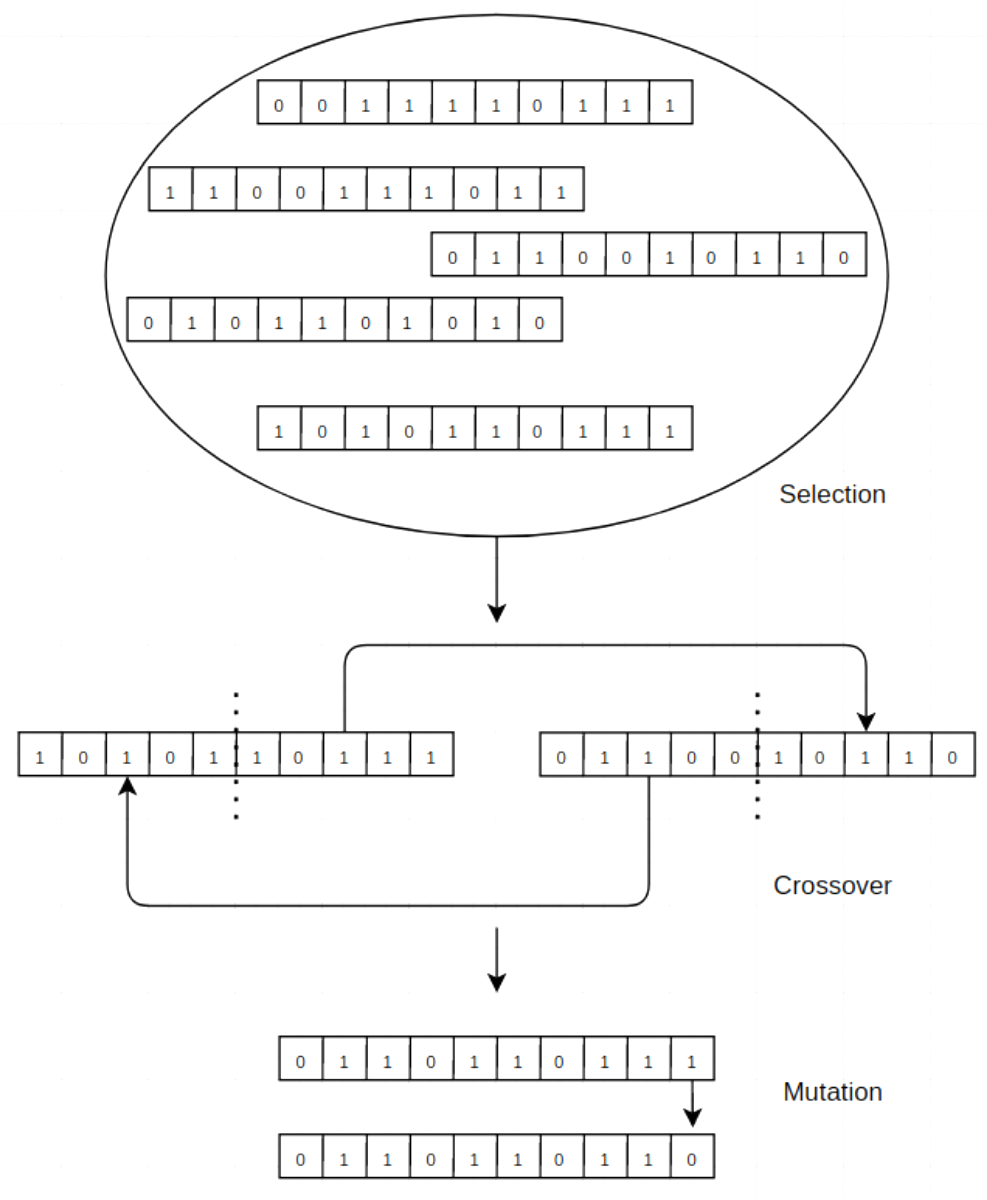
\includegraphics[width=7cm]{p2.png}
\caption{Genetic Operators}
\label{p3}
\end{figure}
As an example consider, initial state as [1 1 1 0 0 0 0 1] and the target state as [1 0 1 0 0 1 0 0]. Applying the concepts discussed previously, a quantum circuit gate is created for this transition and the associated matrix is given by 
{\scriptsize
$$
\begin{bmatrix}
\begin{bmatrix}
-0.14112954-0.16700839j& 0.07983181-0.29873381j\\
-0.25803742+0.38299128j& 0.22384403+0.01717024j\\
0.06272906+0.25203229j& -0.17352533+0.18676704j\\
-0.46040214-0.12675132j& -0.11769043+0.46751876j\\
\end{bmatrix}\\
\begin{bmatrix}
0.31172643+0.14024689j& -0.11225685-0.02087697j\\
0.16743502+0.29588733j&  0.18771276+0.01118339j\\
0.57520561+0.33055889j&  0.13856821-0.24062621j\\
0.15502007-0.07663589j& -0.38171798-0.16226323j\\
\end{bmatrix}\\
\begin{bmatrix}
0.23308965-0.15943424j& 0.26838968-0.17899447j\\
-0.19340125+0.42085285j&-0.1072532 +0.1531806j\\
0.04524549-0.44413067j& 0.15183147-0.24693186j\\
-0.2982411 +0.05650701j&  0.18590532-0.3958033j\\
\end{bmatrix}\\
\begin{bmatrix}
-0.07005404+0.04745812j& -0.27252377-0.17790739j\\
-0.2187864 +0.24156256j& -0.26294328+0.3396825j\\
0.10360916-0.35043418j&  0.12404486+0.42213862j\\
0.44304366-0.02873782j& -0.22363463+0.14806583j\\
\end{bmatrix}\\
\begin{bmatrix}
0.37175985+0.28751052j &-0.07056257-0.1013915j\\  
-0.35527493+0.07918063j & 0.48963077-0.31625964j\\
-0.20088489-0.20871619j &-0.19892169-0.09136702j\\
0.29164278+0.21288127j  &0.08750707+0.14750696j\\
\end{bmatrix}\\
\begin{bmatrix}
-0.38421248-0.04067692j& 0.16637992+0.61802823j\\ 
-0.17373866+0.27097997j& 0.18105618-0.29023612j \\
0.02505396-0.15353303j& 0.11080511+0.16151108j\\
-0.02153527+0.158645j& -0.32556212-0.16206476j\\
\end{bmatrix}\\
\begin{bmatrix}
0.19075161-0.30210472j& -0.09189932-0.2130557j\\  
-0.13117622-0.29864423j&  0.01177846-0.25807943j\\
-0.11828712+0.02111738j&  0.687924  +0.04122678j\\
-0.12997132+0.21518361j& -0.28512878+0.10722509j\\
\end{bmatrix}\\
\begin{bmatrix}
0.50059262+0.00708867j& -0.01602864+0.44984401j\\  
0.01398646+0.08782445j& -0.25293655+0.32748978j\\
-0.13217757+0.13982117j& -0.11740198+0.07269765j\\
-0.1949218 +0.44227633j& -0.09510568+0.26242716j\\
\end{bmatrix}\\
\end{bmatrix}
$$
}
\subsection{Key Points}
Some of the important points governing the flow of the algorithm are mentioned below:

\begin{itemize}
\item The input chromosomes provided are in the form of a bit vector, which is later translated to a quantum register i.e, $\psi$ = $\psi\textsubscript{1} \oplus \psi\textsubscript{2} \oplus \dots \psi\textsubscript{n}$. The $\oplus$ operator is called the tensorial product in the Hilbert space.

\item The most important characteristic of this endeavor is the ability of both the sub-algorithm to retain information. For the evolutionary part, it is the lower swarm particles who memorize the pitfalls. Information retention in QC is guaranteed by the No-Hiding Theorem. The No-Hiding Theorem in an enlarged Hilbert space is given in Equation $\ref{eq:4}$. Due to the correlation between subsystems, quantum information cannot be lost. 

\begin{equation}
\label{eq:4}
\begin{split}
\ket{\mu} \otimes \ket{A} & \rightarrow \sum_{k}^{}\sqrt{p\textsubscript{k}}\ket{k} \otimes \ket{A\textsubscript{k}(\psi)}\\
& = \sum_{k}^{}\sqrt{p\textsubscript{k}}\ket{k} \otimes (\ket{q\textsubscript{k}} \otimes \ket{psi} \otimes 0)
\end{split}
\end{equation}

\item The unused dimension of the Hilbert space is filled by $\otimes 0$ vectors. These unused dimensions can be utilized to completely hide a subsystem and hence delete the information.
\end{itemize}

\subsection{QC Critical Factor: Schema Theorem}
The Schema Theorem \cite{st} dictates which chromosomes move on through the selection phase. If we consider each chromosome as a binary string, there are three possibilities for each bit. It can either be a 1, or a 0 or a * (wildcard) value. The wildcard bit can have either a 1 or a 0. There are two defining characteristics that dictate the goodness of fit. 

\begin{itemize}
\item Order: Number of non-wildcard bits 
\item Defining Length: Distance between two furthermost non-wildcard bits
\end{itemize}

For eg, a chromosome '*10**01' will have an order of 4 and a defining length of 5. This particular chromosome represents the set of chromosomes that have a 0 or 1 in the leftmost bit, followed by a 10, then two wildcards and ends with a 01. The initial population corresponds to multiple schemata and over the course of applying the genetic operators, some survive while others survive. According to the schema theorem, schemata to low order, high fitness, and short defining length reappear in future generations. For a better understanding, an analogy can be drawn between the schema and matching expressions using regular expressions in programming constructs.


\subsection{EC Critical Factor: Fitness Selection}
The evolutionary algorithm depends greatly on the quality of the fitness function \cite{haram}. It forms the basis for the next generation. In CC, a tailor-made fitness function might suffice for each problem. But for a self-organizing QC system, the main program would have to run multiple times to determine the fitness from each output. Even if a real quantum computer was used, we would get one output and it's associated probability from each epoch. The probability of error so obtained could then be utilized to function as a fitness function. The only drawback in this method would be the absence of a quantum computer and the result of exponential computational resources. 

The probability of error, in itself, is inadequate to function as a fitness function for a QC system. This is due to the extreme ease with which a program could be produced with a 50\% best-case accuracy that is nowhere close to the real output. As an analogy, the construction of such a program to decide the circuit would be like tossing a coin to decide the next gate in the circuit. 

The function used in this paper is a combination of the probability of error and a count of the number of fitness cases for which the program produces better results in more than 50\% of the cases. Multiple calls can be made to the "Oracle" to minimize the number of gates in the circuit. Other quantum mechanical properties could also be utilized for improved fitness functions. 


\section{Results and Discussion}

\subsection{Experimental Setup}
Due to the unavailability of a quantum computer, an artificial environment was created and simulations were conducted in it. The experiment was set up on a 64-bit Machine with Ubuntu 20.04, Intel® CoreTM i5-7200U CPU @ 2.50GHz × 4, with a GeForce 940MX/PCle/SSE2 graphic card. 

To design a quantum state system, we provide the program with a set of input qubits mapped to a set of output qubits. As discussed previously the fitness function is chosen as a lexicographic combination of the number of misses and probability of error as given in Equation $\ref{eq:5}$, where $\alpha$ is a scaling factor, $\textit{m}$ is the number of misses, and $\textit{e}$ is the probability of error \cite{lex}. The lower the value returned by the fitness function, the higher is the solution's quality.

\begin{equation}
\label{eq:5}
f = \alpha m + e
\end{equation}


\subsection{Results}
Following this, an initial set of chromosomes corresponding to the ideal circuit were created and gently evolved for a set number of generations. The generation progression is composed of the previously mentioned genetic operators. A global count of the best fitness achieved for far is mentioned and the matrix corresponding to that score is declared as the optimal circuit design \cite{cir}. The results have been composed for 100 generations in 10 test runs and displayed in Table $\ref{tab:3}$.  


\begin{table*}[!t]
\caption{\textsc{Results}}
\label{tab:3}
\centering
{
\begin{tabular}{| c | c | c | c | c |}
\hline
Experiment No. & Input Qubit & Output Qubit & Number of Chromosomes &  Best Fitness Value \\
\hline
 & [0 1 1 1 0 1 0 0] & [0 0 0 0 1 1 1 1] & 10 & 0.5081 \\
1 & [0 1 1 1 0 1 0 0] & [0 0 0 0 1 1 1 1] & 50 & 0.5134 \\
 & [0 1 1 1 0 1 0 0] & [0 0 0 0 1 1 1 1] & 100 & 0.5106 \\
\hline
 & [0 1 1 0 0 1 1 1] & [0 0 1 0 1 0 1 1] & 10 & 0.4366 \\
2 & [0 1 1 0 0 1 1 1] & [0 0 1 0 1 0 1 1] & 50 & 0.4821 \\
 & [0 1 1 0 0 1 1 1] & [0 0 1 0 1 0 1 1] & 100 & 0.4911 \\
\hline
 & [1 0 1 1 1 1 1 1] & [0 1 1 0 0 1 1 0] & 10 & 0.3985 \\
3 & [1 0 1 1 1 1 1 1] & [0 1 1 0 0 1 1 0] & 50 & 0.3672 \\
 & [1 0 1 1 1 1 1 1] & [0 1 1 0 0 1 1 0] & 100 & 0.3725 \\
\hline
 & [1 0 1 1 1 1 0 1] & [1 1 0 1 0 1 0 0] & 10 & 0.4786 \\
4 & [1 0 1 1 1 1 0 1] & [1 1 0 1 0 1 0 0] & 50 & 0.4332 \\
 & [1 0 1 1 1 1 0 1] & [1 1 0 1 0 1 0 0] & 100 & 0.4189 \\
\hline
 & [1 0 0 1 1 0 0 0] & [0 1 0 1 0 1 1 0] & 10 & 0.6444 \\
5 & [1 0 0 1 1 0 0 0] & [0 1 0 1 0 1 1 0] & 50 & 0.5842 \\
 & [1 0 0 1 1 0 0 0] & [0 1 0 1 0 1 1 0] & 100 & 0.6179 \\
\hline
 & [1 0 0 1 1 0 0 0] & [1 1 1 1 0 0 0 0] & 10 & 0.4615 \\
6 & [1 0 0 1 1 0 0 0] & [1 1 1 1 0 0 0 0] & 50 & 0.4311 \\
 & [1 0 0 1 1 0 0 0] & [1 1 1 1 0 0 0 0] & 100 & 0.4872 \\
\hline
 & [0 0 1 0 1 1 1 0] & [0 1 0 0 0 0 0 1] & 10 & 0.5895 \\
7 & [0 0 1 0 1 1 1 0] & [0 1 0 0 0 0 0 1] & 50 & 0.6294 \\
 & [0 0 1 0 1 1 1 0] & [0 1 0 0 0 0 0 1] & 100 & 0.5574 \\
\hline
 & [0 0 1 1 0 1 0 1] & [1 1 1 0 0 1 1 0] & 10 & 0.4689 \\
8 & [0 0 1 1 0 1 0 1] & [1 1 1 0 0 1 1 0] & 50 & 0.4355 \\
 & [0 0 1 1 0 1 0 1] & [1 1 1 0 0 1 1 0] & 100 & 0.4476 \\
\hline
 & [0 0 0 0 0 1 1 0] & [1 0 1 1 1 1 0 1] & 10 & 0.5610 \\
9 & [0 0 0 0 0 1 1 0] & [1 0 1 1 1 1 0 1] & 50 & 0.5812 \\
 & [0 0 0 0 0 1 1 0] & [1 0 1 1 1 1 0 1] & 100 & 0.4877 \\
\hline
 & [0 1 1 1 0 0 0 0] & [1 1 1 1 1 0 0 1] & 10  & 0.4919 \\
10 & [0 1 1 1 0 0 0 0] & [1 1 1 1 1 0 0 1] & 50  & 0.4682 \\
 & [0 1 1 1 0 0 0 0] & [1 1 1 1 1 0 0 1] & 100  & 0.4158 \\
\hline
\end{tabular}
}
\end{table*}

As we can see, the results for test runs 1, 5, 7, and 9 are extremely promising. Further fine-tuning could be applied to narrow down the chromosome population. These results act as proof-of-concept when it comes to combing the field of computational intelligence with quantum mechanics. 

\subsection{Conclusion and Future Scope}

Applied automatic programming technologies with the discovery of new quantum speedups in genetic programming systems are an extremely promising avenue and are worthy of serious investigation. Construction of large scale quantum computers can leverage the unprecedented computational powers offered by EQUATe and the results so listed, act as a proof-of-concept. The main area of improvement for EQUATe would involve identifying and realizing the "embarrassingly parallel" EC methods and run them on accelerated high-performance computing clusters. Similarly parallelizing the QC component of EQUATe will result in a decreased memory footprint leading to optimal memory allocation and utilization.

\begin{thebibliography}{00}

\bibitem{hara}T. Harada, "Mathematical Model of Asynchronous Parallel Evolutionary Algorithm to Analyze Influence of Evaluation Time Bias," 2019 IEEE Asia-Pacific Conference on Computer Science and Data Engineering (CSDE), Melbourne, Australia, 2019, pp. 1-8, doi: 10.1109/CSDE48274.2019.9162360.

\bibitem{mul} J. J. Liang, C. T. Yue and B. Y. Qu, "Multimodal multi-objective optimization: A preliminary study," 2016 IEEE Congress on Evolutionary Computation (CEC), Vancouver, BC, 2016, pp. 2454-2461, doi: 10.1109/CEC.2016.7744093.

\bibitem{pare} P. Ngatchou, A. Zarei and A. El-Sharkawi, "Pareto Multi Objective Optimization," Proceedings of the 13th International Conference on, Intelligent Systems Application to Power Systems, Arlington, VA, 2005, pp. 84-91, doi: 10.1109/ISAP.2005.1599245.

\bibitem{az} A. Zeilinger, "Quantum entanglement and information," Quantum Electronics and Laser Science Conference (QELS 2000). Technical Digest. Postconference Edition. TOPS Vol.40 (IEEE Cat. No.00CH37089), San Francisco, CA, USA, 2000, pp. 163-.

\bibitem{vik} P. A. Vikhar, "Evolutionary algorithms: A critical review and its future prospects," 2016 International Conference on Global Trends in Signal Processing, Information Computing and Communication (ICGTSPICC), Jalgaon, 2016, pp. 261-265, doi: 10.1109/ICGTSPICC.2016.7955308.

\bibitem{self} H-G. Beyer and K. Deb, "On self-adaptive features in real-parameter evolutionary algorithms," in IEEE Transactions on Evolutionary Computation, vol. 5, no. 3, pp. 250-270, June 2001, doi: 10.1109/4235.930314.


\bibitem{oracle} J. Chen et al., "Supporting oracle construction via static analysis," 2016 31st IEEE/ACM International Conference on Automated Software Engineering (ASE), Singapore, 2016, pp. 178-189.

\bibitem{qg} P. I. Hagouel and I. G. Karafyllidis, "Quantum computers: Registers, gates and algorithms," 2012 28th International Conference on Microelectronics Proceedings, Nis, 2012, pp. 15-21, doi: 10.1109/MIEL.2012.6222789.

\bibitem{gwo} D. Jitkongchuen, P. Phaidang and P. Pongtawevirat, "Grey wolf optimization algorithm with invasion-based migration operation," 2016 IEEE/ACIS 15th International Conference on Computer and Information Science (ICIS), Okayama, 2016, pp. 1-5, doi: 10.1109/ICIS.2016.7550769.

\bibitem{st} Liang Ming, Yu-Ping Wang and Yu-ming Cheung, "A new schema theorem for uniform crossover based on ternary representation," Proceedings of the 2004 Intelligent Sensors, Sensor Networks and Information Processing Conference, 2004., Melbourne, Vic., Australia, 2004, pp. 235-239, doi: 10.1109/ISSNIP.2004.1417468.

\bibitem{haram} M. Harman and J. Clark, "Metrics are fitness functions too," 10th International Symposium on Software Metrics, 2004. Proceedings., Chicago, Illinois, USA, 2004, pp. 58-69, doi: 10.1109/METRIC.2004.1357891.

\bibitem{lex} T. Zheng, G. Wu and D. He, "Nonlinear model predictive control based on lexicographic multi-objective genetic algorithm," 2007 International Conference on Intelligent and Advanced Systems, Kuala Lumpur, 2007, pp. 61-65, doi: 10.1109/ICIAS.2007.4658348.

\bibitem{cir}Z. Vasicek and L. Sekanina, "Evolutionary Approach to Approximate Digital Circuits Design," in IEEE Transactions on Evolutionary Computation, vol. 19, no. 3, pp. 432-444, June 2015, doi: 10.1109/TEVC.2014.2336175.
\end{thebibliography}

\end{document}
